\documentclass[12pt,a4paper]{article}
\usepackage[a4paper,margin=1in]{geometry}
\usepackage{graphicx}
\usepackage{booktabs}
\usepackage{amsmath,amssymb}
\usepackage{float}
\usepackage{hyperref}
\usepackage{xcolor}
\usepackage{listings}
\usepackage{enumitem}
\usepackage{fancyhdr}
\usepackage{longtable}
\usepackage{array}
\hypersetup{colorlinks=true,linkcolor=blue,urlcolor=blue}
\pagestyle{fancy}
\fancyhf{}
\lhead{ICS1512}
\rhead{Machine Learning Algorithms Laboratory}
\cfoot{\thepage}
\lstset{language=Python,basicstyle=\ttfamily\small,numbers=left,frame=single,breaklines=true,showstringspaces=false}
\begin{document}

\begin{tabular}{|p{4cm}|p{11cm}|}
\hline
Experiment No. & 5 \\ \hline
Experiment Title & Decision Tree and Random Forest: A Comparative Classification Study \\ \hline
Student Name & Harshitaa B \\ \hline
Register Number & 3122247001021\\ \hline
Faculty & Dr. Poreddy Ajay Kumar Reddy \\ \hline
Due Date & 16th August 2026\\ \hline
\end{tabular}

\vspace{0.4cm}
\noindent\textbf{Institution:} Sri Sivasubramaniya Nadar College of Engineering, Chennai\\
\textbf{Programme:} M.Tech (Integrated) Computer Science \& Engineering\\
\textbf{Semester:} V\\
\textbf{Subject:} ICS1512 \& Machine Learning Algorithms Laboratory\\
\textbf{Academic Year:} 2026--2027 (Odd)\\
\textbf{Batch:} 2024--2029\\
\textbf{Dataset:} Wisconsin Diagnostic Breast Cancer Dataset

\section{Objective}
\begin{itemize}
\item To implement a Decision Tree classifier.
\item To extend the Decision Tree into a Random Forest ensemble model.
\item To study the impact of hyperparameters on overfitting and generalization.
\item To select optimal hyperparameters using 5-Fold Cross-Validation.
\item To compare single-tree and ensemble-tree models.
\end{itemize}

\section{Problem Statement}
The task is to classify observations from the Wisconsin Diagnostic Breast Cancer dataset into malignant and benign classes. A Decision Tree and a Random Forest classifier are trained, tuned using stratified 5-fold cross-validation, and evaluated on a held-out 20\% test set. The experiment studies tree complexity, ensemble hyperparameters, overfitting, stability, and generalization.

\section{Dataset Description}
\begin{longtable}{|p{6cm}|p{8cm}|}
\hline
Dataset Name & Wisconsin Diagnostic Breast Cancer (WDBC) Dataset \\ \hline
Dataset Source & UCI Machine Learning Repository / scikit-learn dataset copy \\ \hline
Number of Samples & 569 \\ \hline
Number of Features & 30 numerical attributes \\ \hline
Number of Classes & 2: Malignant (M) and Benign (B) \\ \hline
Missing Values & None in the supplied dataset \\ \hline
Train-Test Split & 80\% training, 20\% testing; stratified \\ \hline
\end{longtable}

\section{Exploratory Data Analysis}
The notebook performs dataset overview, descriptive statistics, missing-value analysis, class-distribution analysis, and feature-correlation analysis.

\subsection{Class Distribution}
\begin{figure}[H]\centering

\includegraphics[width=0.70\linewidth]{figs/class_distribution.png}
\caption{Class distribution of the WDBC dataset.}
\end{figure}
\textbf{Inference:} The two target classes have different frequencies. Stratified splitting and cross-validation preserve class proportions and make the model comparison more consistent.

\subsection{Feature Correlation}
\begin{figure}[H]\centering

\includegraphics[width=0.90\linewidth]{figs/correlation_matrix.png}
\caption{Correlation matrix of the 30 numerical features.}
\end{figure}
\textbf{Inference:} Several measurements are strongly correlated because they describe related properties of cell nuclei. Decision Trees and Random Forests do not require feature scaling. Random Forest additionally uses random feature subsets to increase tree diversity.

\section{Data Preprocessing}
\begin{itemize}
\item No missing-value imputation is required because the dataset contains no missing values in the supplied representation.
\item The target is binary and is mapped to Malignant and Benign for interpretation.
\item Feature scaling is not required for tree-based models.
\item An 80--20 stratified train-test split is used.
\item No additional feature engineering is applied.
\end{itemize}

\section{Machine Learning Algorithm}

\subsection{Decision Tree Classifier}
A Decision Tree recursively splits the feature space using impurity reduction. For class probabilities $p_1,\ldots,p_K$, Gini impurity is
\[
G=1-\sum_{k=1}^{K}p_k^2,
\]
while entropy is
\[
H=-\sum_{k=1}^{K}p_k\log_2(p_k).
\]
A tree chooses splits that improve node purity. Greater depth permits more complex decision rules but can increase variance and overfitting.

\textbf{Advantages:} easy interpretation, no scaling requirement, and ability to model nonlinear relationships.

\textbf{Limitations:} sensitivity to training-data changes, high variance, and overfitting when grown excessively deep.

\subsection{Random Forest Classifier}
Random Forest combines many decision trees trained using randomized observations and feature subsets. For classification,
\[
\hat y(x)=\operatorname{mode}\{\hat y_1(x),\hat y_2(x),\ldots,\hat y_B(x)\}.
\]
Bootstrap sampling and random feature selection reduce correlation among individual trees, while aggregation reduces variance.

\textbf{Advantages:} improved stability, reduced variance, nonlinear modelling, and strong generalization in many tabular settings.

\textbf{Limitations:} greater computational cost and reduced direct interpretability compared with one tree.

\section{Experimental Setup}
\begin{tabular}{ll}
\toprule
Python Version & Recorded by notebook at runtime\\
Scikit-Learn Version & Recorded by notebook at runtime\\
IDE & Jupyter Notebook / JupyterLab\\
Operating System & Recorded by notebook at runtime\\
Hardware & Recorded by notebook at runtime\\
Random State & 42\\
Cross-Validation & Stratified 5-Fold\\
Test Size & 20\%\\
\bottomrule
\end{tabular}

\section{Hyperparameter Selection}
\subsection{Decision Tree}
The search space includes criterion (Gini, entropy, log loss), maximum depth (2, 3, 4, 5, 7, 10, unrestricted), minimum samples split (2, 5, 10), and minimum samples leaf (1, 2, 4).

\subsection{Random Forest}
The search space includes number of estimators (50, 100, 200), maximum depth (unrestricted, 5, 10, 15), maximum features (sqrt, log2, all), and bootstrap (True/False).

The search uses stratified 5-fold cross-validation. Mean F1-score is used as the refit criterion, while mean accuracy is also recorded.

```latex
\section{Hyperparameter Tuning Results}

\begin{table}[H]\centering
\caption{Decision Tree Hyperparameter Evaluation using 5-Fold Cross-Validation}
\begin{tabular}{lcccc}
\toprule
Criterion & Max Depth & Avg CV Accuracy (\%) & Avg CV F1 Score (\%)\\
\midrule
Gini & 5 & 93.85 & 95.06\\
\bottomrule
\end{tabular}
\end{table}

Best parameters:
\texttt{\{'criterion': 'gini', 'max\_depth': 5, 'min\_samples\_leaf': 4, 'min\_samples\_split': 2\}}

Best mean CV F1: 0.95058

\begin{table}[H]\centering
\caption{Random Forest Hyperparameter Evaluation using 5-Fold Cross-Validation}
\begin{tabular}{ccccc}
\toprule
n estimators & Max Depth & Max Features & Avg CV Accuracy (\%) & Avg CV F1 Score (\%)\\
\midrule
100 & None & log2 & 96.48 & 97.18\\
\bottomrule
\end{tabular}
\end{table}

Best parameters:
\texttt{\{'bootstrap': True, 'max\_depth': None, 'max\_features': 'log2', 'n\_estimators': 100\}}

Best mean CV F1: 0.97180


\section{5-Fold Cross-Validation Performance Comparison} \begin{table}[H]\centering \caption{5-Fold Cross-Validation Accuracy Comparison} \begin{tabular}{lcccccc} \toprule Model & Fold 1 & Fold 2 & Fold 3 & Fold 4 & Fold 5 & Average\\ \midrule Decision Tree & 0.9451 & 0.9451 & 0.9121 & 0.9231 & 0.9670 & 0.9385\\ Random Forest & 0.9670 & 0.9780 & 0.9341 & 0.9560 & 0.9890 & 0.9648\\ \bottomrule \end{tabular} \end{table}

\section{Results}

\begin{table}[H]\centering
\caption{Final Evaluation Metrics on the Held-Out Test Set}
\begin{tabular}{lccccc}
\toprule
Model & Accuracy & Precision & Recall & F1 Score & ROC-AUC\\
\midrule
Decision Tree & 0.9035 & 0.9420 & 0.9028 & 0.9220 & 0.9358\\
Random Forest & 0.9561 & 0.9589 & 0.9722 & 0.9655 & 0.9924\\
\bottomrule
\end{tabular}
\end{table}
```

\section{Result Visualization}

\subsection{Decision Tree Depth}
\begin{figure}[H]\centering
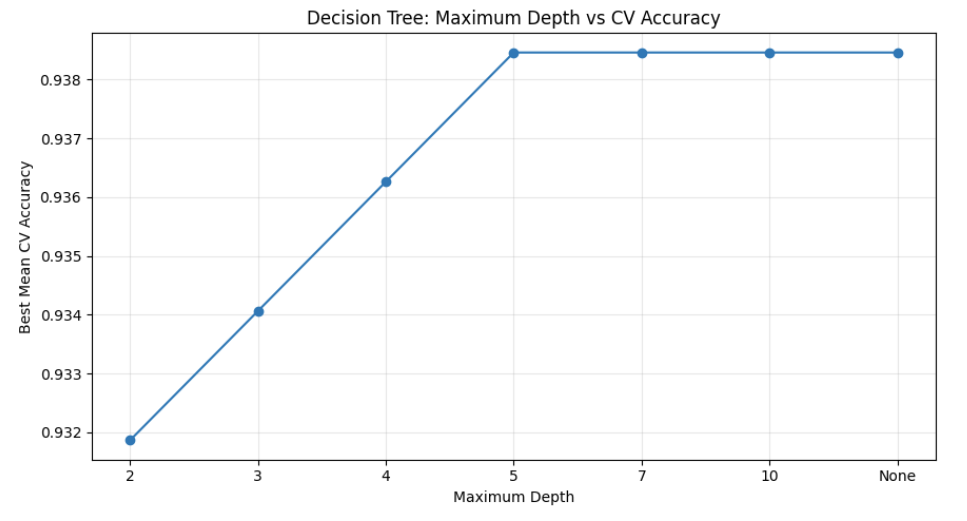
\includegraphics[width=0.80\linewidth]{figs/decision_tree_depth_effect.png}
\caption{Maximum depth versus best cross-validation accuracy for the Decision Tree.}
\end{figure}
\textbf{Inference:} Depth controls tree complexity. Shallow trees can underfit, while excessive depth can increase variance. Cross-validation provides an empirical basis for selecting a suitable depth.

\subsection{Decision Tree Structure}
\begin{figure}[H]\centering
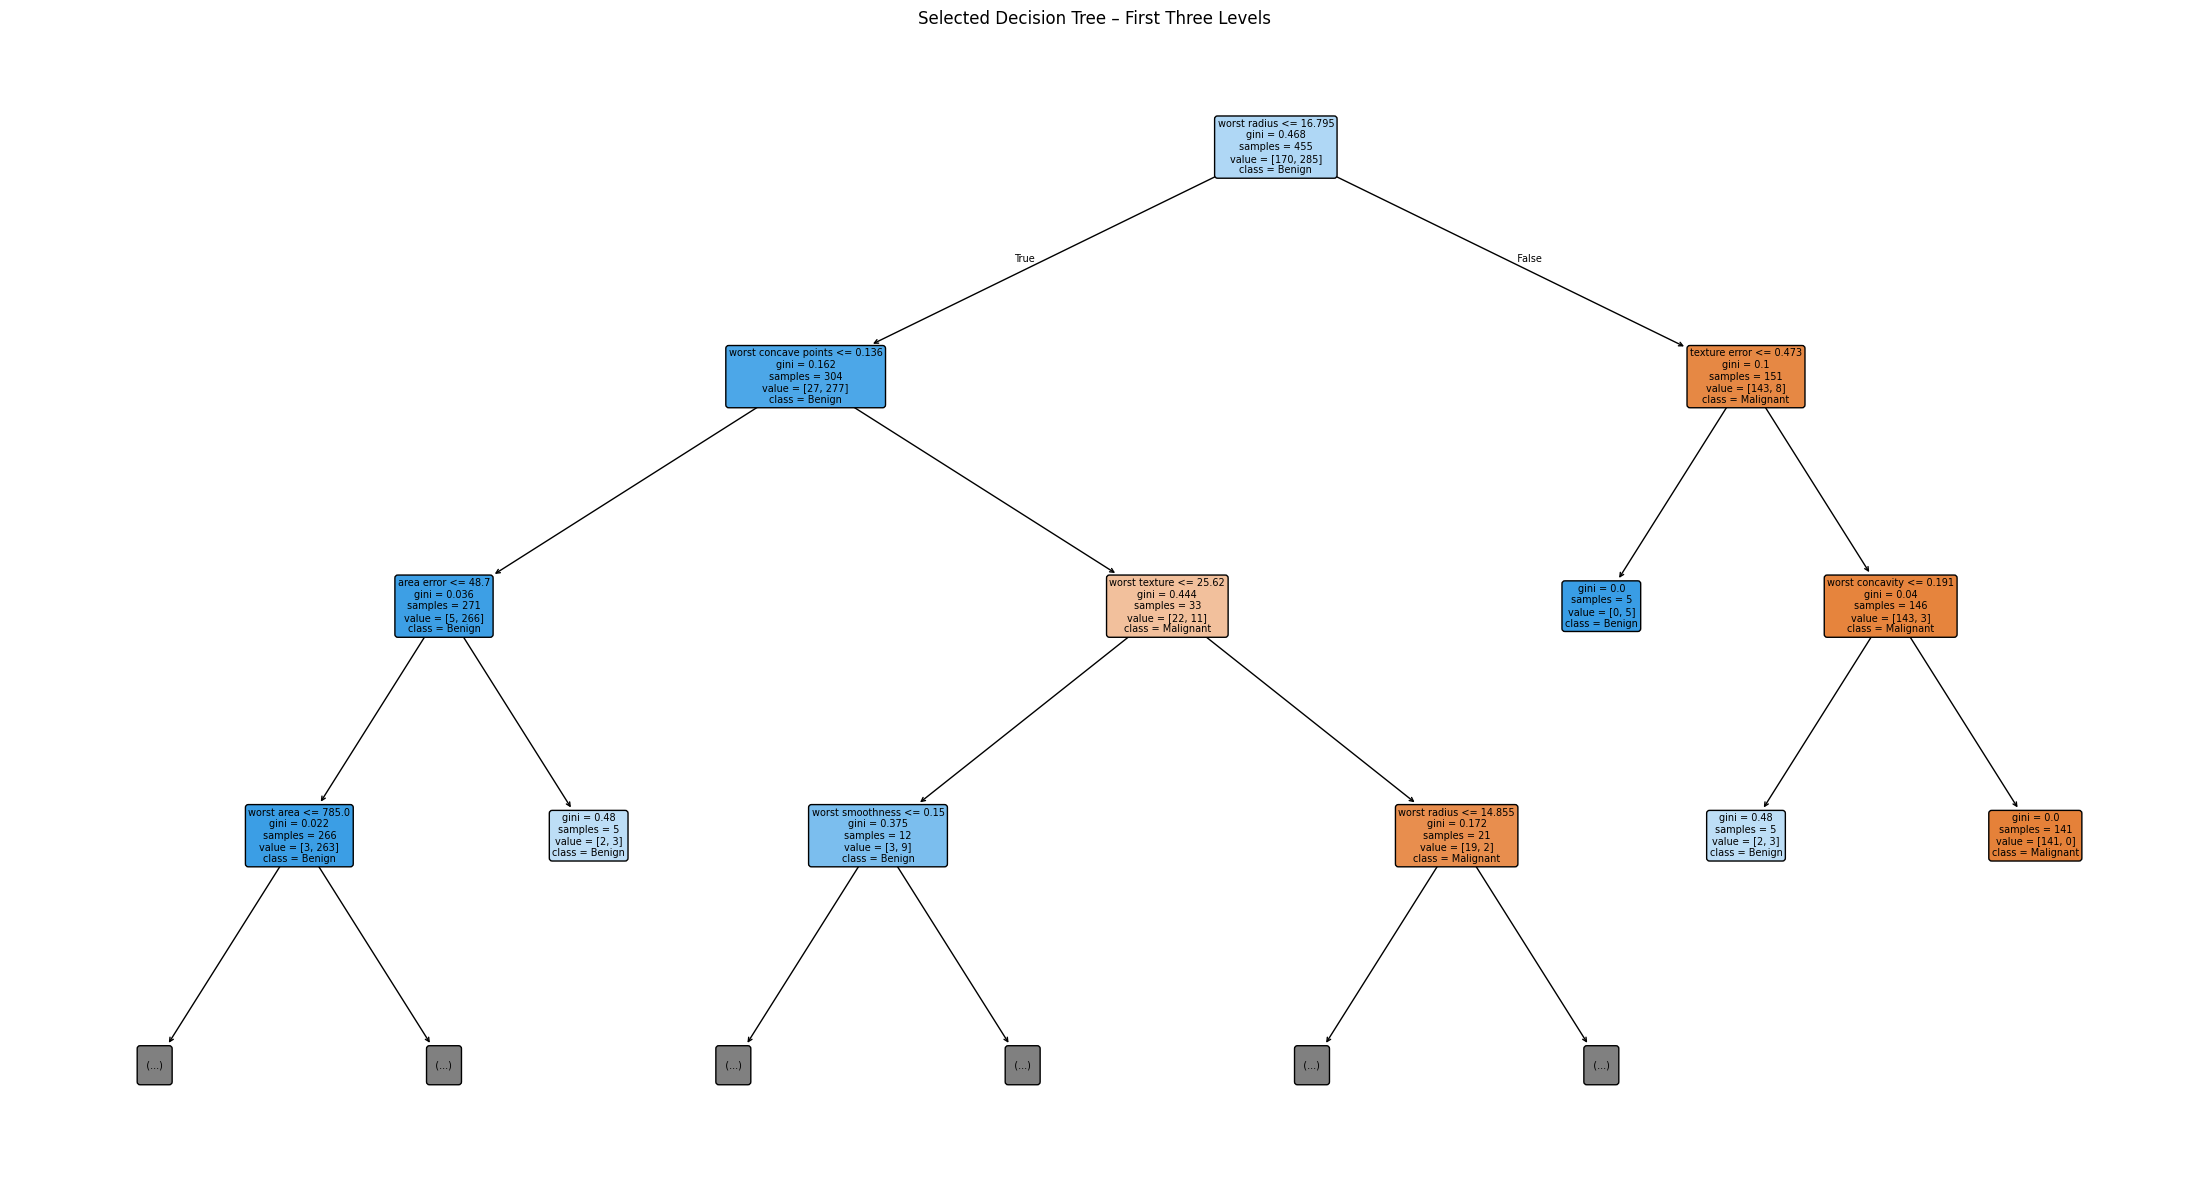
\includegraphics[width=0.75\linewidth]{figs/decision_tree_levels.png}
\caption{First three levels of the selected Decision Tree.}
\end{figure}
\textbf{Inference:} The tree shows how feature thresholds recursively divide the observations. The displayed first three levels provide an interpretable view of the learned decision rules.

\subsection{Random Forest Number of Estimators}
\begin{figure}[H]\centering
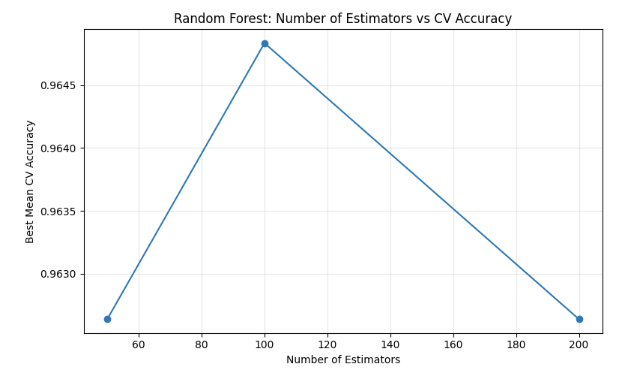
\includegraphics[width=0.80\linewidth]{figs/random_forest_estimators_effect.png}
\caption{Number of Random Forest estimators versus best cross-validation accuracy.}
\end{figure}
\textbf{Inference:} More trees can stabilize predictions by aggregating more randomized learners. Performance may reach a plateau, producing diminishing returns for additional trees.

\subsection{Decision Tree Confusion Matrix}
\begin{figure}[H]\centering
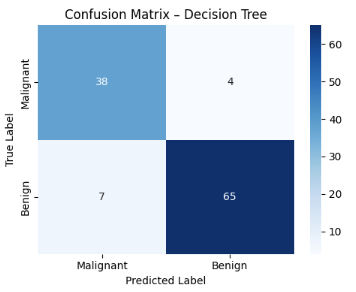
\includegraphics[width=0.65\linewidth]{figs/decision_tree_confusion_matrix.png}
\caption{Confusion matrix for the selected Decision Tree.}
\end{figure}
\textbf{Inference:} The matrix shows correct and incorrect predictions by class. It complements aggregate metrics by revealing the distribution of false positives and false negatives.

\subsection{Random Forest Confusion Matrix}
\begin{figure}[H]\centering
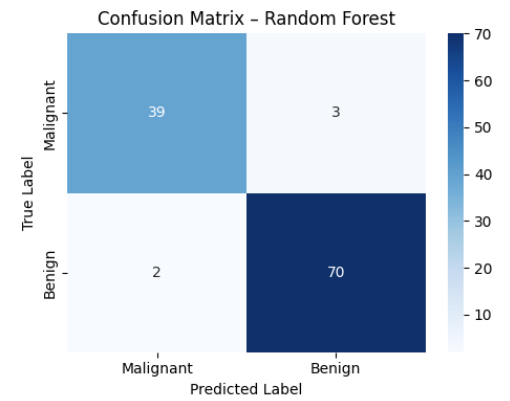
\includegraphics[width=0.65\linewidth]{figs/random_forest_confusion_matrix.png}
\caption{Confusion matrix for the selected Random Forest.}
\end{figure}
\textbf{Inference:} The Random Forest matrix provides class-specific information about its errors. Comparing it with the Decision Tree matrix shows how ensemble aggregation changes prediction behaviour.

\subsection{ROC Curve}
\begin{figure}[H]\centering
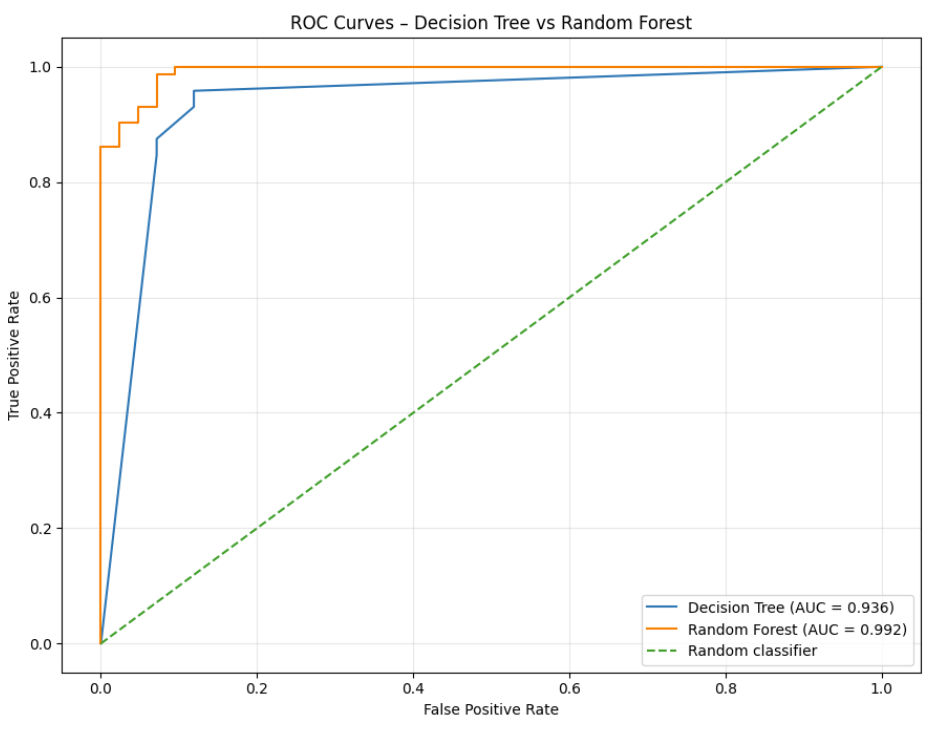
\includegraphics[width=0.85\linewidth]{figs/roc_curves.png}
\caption{ROC curves comparing Decision Tree and Random Forest.}
\end{figure}
\textbf{Inference:} ROC curves show the trade-off between true-positive and false-positive rates across thresholds. AUC summarizes discrimination across those thresholds.

\subsection{Random Forest Feature Importance}
\begin{figure}[H]\centering
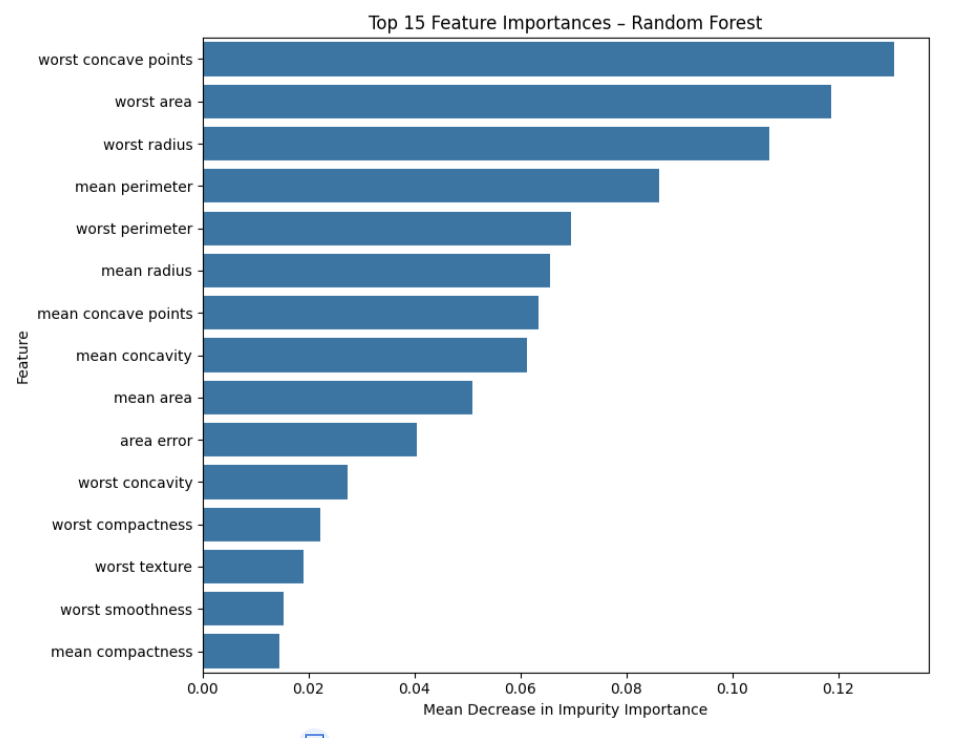
\includegraphics[width=0.85\linewidth]{figs/random_forest_feature_importance.png}
\caption{Top 15 Random Forest feature importances.}
\end{figure}
\textbf{Inference:} Feature importance identifies variables that contribute strongly to tree splitting in the fitted forest. These values are model-specific and do not imply causality.

\section{Discussion}
\subsection{Effect of Tree Depth}
Increasing depth allows increasingly complex decision rules. Training error can decrease as depth increases, but a very deep tree can model noise and increase variance. Cross-validation helps select a more appropriate complexity level.

\subsection{Hyperparameter Impact}
Decision Tree performance is influenced by criterion, maximum depth, minimum samples split, and minimum samples leaf. Random Forest performance depends on ensemble size, tree depth, feature subsampling, and bootstrap sampling. The GridSearchCV tables provide the empirical comparison of these settings.

\subsection{Generalization}
Random Forest improves stability by averaging many randomized trees. Bootstrap sampling gives trees different training samples, while random feature selection reduces correlation among trees. This generally reduces variance relative to a single high-variance Decision Tree.

\subsection{Does Ensemble Learning Always Improve Performance?}
No fixed improvement should be assumed before observing the results. The ensemble may improve some metrics while not improving every metric on a particular finite test set. Dataset characteristics, tree diversity, hyperparameters, and sampling variation all influence the outcome.

\section{Observation Questions}
\subsection*{1. How does tree depth affect overfitting in Decision Trees?}
Greater depth increases model complexity. Shallow trees may underfit, whereas very deep trees may fit noise and training-specific patterns, increasing variance. Cross-validation helps select a suitable depth.

\subsection*{2. Which hyperparameter had the greatest impact on performance?}
This should be determined from the actual GridSearchCV results. Compare the validation scores across criterion, maximum depth, minimum samples split, and minimum samples leaf for the Decision Tree, and across number of estimators, maximum depth, maximum features, and bootstrap for Random Forest.

\subsection*{3. How does Random Forest improve generalization?}
It combines many trees trained with bootstrap samples and random feature subsets. Aggregating diverse trees reduces dependence on any individual high-variance tree and can improve stability on unseen data.

\subsection*{4. Did ensemble learning always improve performance? Why or why not?}
Use the measured cross-validation and test-set metrics to answer this. Ensemble learning does not guarantee improvement on every finite test set or every metric; its benefit depends on model diversity, hyperparameters, dataset structure, and sampling variability.

\section{Conclusion}
Decision Tree and Random Forest classifiers were implemented and evaluated on the Wisconsin Diagnostic Breast Cancer dataset. Hyperparameters were selected using stratified 5-fold cross-validation, and final performance was measured on an independent 20\% test set. The experiment demonstrates how tree complexity affects overfitting and how Random Forest uses bootstrap sampling, random feature selection, and aggregation to reduce variance and improve stability.

\section{References}
\begin{enumerate}[label={[}\arabic*{]}]
\item Scikit-learn, ``Decision Trees,'' \url{https://scikit-learn.org/stable/modules/tree.html}.
\item Scikit-learn, ``Ensemble Methods / Random Forest,'' \url{https://scikit-learn.org/stable/modules/ensemble.html}.
\item UCI Machine Learning Repository, ``Breast Cancer Wisconsin (Diagnostic) Dataset,'' \url{https://archive.ics.uci.edu/}.
\item F. Pedregosa et al., ``Scikit-learn: Machine Learning in Python,'' \textit{Journal of Machine Learning Research}, vol. 12, pp. 2825--2830, 2011.
\end{enumerate}
\end{document}
